\documentclass[journal,oneside,a4paper,onecolumn]{IEEEtran}

% Some very useful LaTeX packages include:
% (uncomment the ones you want to load)

% *** CITATION PACKAGES ***
%
\usepackage{cite}
% cite.sty was written by Donald Arseneau
% V1.6 and later of IEEEtran pre-defines the format of the cite.sty package
% \cite{} output to follow that of IEEE. Loading the cite package will
% result in citation numbers being automatically sorted and properly
% "compressed/ranged". e.g., [1], [9], [2], [7], [5], [6] without using
% cite.sty will become [1], [2], [5]--[7], [9] using cite.sty. cite.sty's
% \cite will automatically add leading space, if needed. Use cite.sty's
% noadjust option (cite.sty V3.8 and later) if you want to turn this off.
% cite.sty is already installed on most LaTeX systems. Be sure and use
% version 4.0 (2003-05-27) and later if using hyperref.sty. cite.sty does
% not currently provide for hyperlinked citations.
% The latest version can be obtained at:
% http://www.ctan.org/tex-archive/macros/latex/contrib/cite/
% The documentation is contained in the cite.sty file itself.


% *** GRAPHICS RELATED PACKAGES ***
%
  \usepackage{graphicx}
  \graphicspath{{figs/}}
  \DeclareGraphicsExtensions{.pdf,.png}
  \usepackage{color}

% *** MATH PACKAGES ***
%
\usepackage[cmex10]{amsmath}
% A popular package from the American Mathematical Society that provides
% many useful and powerful commands for dealing with mathematics. If using
% it, be sure to load this package with the cmex10 option to ensure that
% only type 1 fonts will utilized at all point sizes. Without this option,
% it is possible that some math symbols, particularly those within
% footnotes, will be rendered in bitmap form which will result in a
% document that can not be IEEE Xplore compliant!
%
% Also, note that the amsmath package sets \interdisplaylinepenalty to 10000
% thus preventing page breaks from occurring within multiline equations. Use:
%\interdisplaylinepenalty=2500
% after loading amsmath to restore such page breaks as IEEEtran.cls normally
% does. amsmath.sty is already installed on most LaTeX systems. The latest
% version and documentation can be obtained at:
% http://www.ctan.org/tex-archive/macros/latex/required/amslatex/math/

%\usepackage{amssymb}%............................ AMS Symbol fonts



% *** SPECIALIZED LIST PACKAGES ***
%
%\usepackage{algorithmic}
% algorithmic.sty was written by Peter Williams and Rogerio Brito.
% This package provides an algorithmic environment for describing algorithms.
% You can use the algorithmic environment in-text or within a figure
% environment to provide for a floating algorithm. Do NOT use the algorithm
% floating environment provided by algorithm.sty (by the same authors) or
% algorithm2e.sty (by Christophe Fiorio) as IEEE does not use dedicated
% algorithm float types and packages that provide these will not provide
% correct IEEE style captions. The latest version and documentation of
% algorithmic.sty can be obtained at:
% http://www.ctan.org/tex-archive/macros/latex/contrib/algorithms/
% There is also a support site at:
% http://algorithms.berlios.de/index.html
% Also of interest may be the (relatively newer and more customizable)
% algorithmicx.sty package by Szasz Janos:
% http://www.ctan.org/tex-archive/macros/latex/contrib/algorithmicx/

% *** ALIGNMENT PACKAGES ***
%
\usepackage{array}
% Frank Mittelbach's and David Carlisle's array.sty patches and improves
% the standard LaTeX2e array and tabular environments to provide better
% appearance and additional user controls. As the default LaTeX2e table
% generation code is lacking to the point of almost being broken with
% respect to the quality of the end results, all users are strongly
% advised to use an enhanced (at the very least that provided by array.sty)
% set of table tools. array.sty is already installed on most systems. The
% latest version and documentation can be obtained at:
% http://www.ctan.org/tex-archive/macros/latex/required/tools/


\usepackage{mdwmath}
\usepackage{mdwtab}
% Also highly recommended is Mark Wooding's extremely powerful MDW tools,
% especially mdwmath.sty and mdwtab.sty which are used to format equations
% and tables, respectively. The MDWtools set is already installed on most
% LaTeX systems. The lastest version and documentation is available at:
% http://www.ctan.org/tex-archive/macros/latex/contrib/mdwtools/

% IEEEtran contains the IEEEeqnarray family of commands that can be used to
% generate multiline equations as well as matrices, tables, etc., of high
% quality.

% *** SUBFIGURE PACKAGES ***
% subfig.sty, also written by Steven Douglas Cochran, is the modern
% replacement for subfigure.sty. However, subfig.sty requires and
% automatically loads Axel Sommerfeldt's caption.sty which will override
% IEEEtran.cls handling of captions and this will result in nonIEEE style
% figure/table captions. To prevent this problem, be sure and preload
% caption.sty with its "caption=false" package option. This is will preserve
% IEEEtran.cls handing of captions. Version 1.3 (2005/06/28) and later
% (recommended due to many improvements over 1.2) of subfig.sty supports
% the caption=false option directly:
\usepackage[caption=false,font=footnotesize]{subfig}
%
% The latest version and documentation can be obtained at:
% http://www.ctan.org/tex-archive/macros/latex/contrib/subfig/
% The latest version and documentation of caption.sty can be obtained at:
% http://www.ctan.org/tex-archive/macros/latex/contrib/caption/

%Setting captions to centered (Not IEEE journal standard)
\makeatletter
\long\def\@makecaption#1#2{\ifx\@captype\@IEEEtablestring%
\footnotesize\begin{center}{\normalfont\footnotesize #1}\\
{\normalfont\footnotesize\scshape #2}\end{center}%
\@IEEEtablecaptionsepspace
\else
\@IEEEfigurecaptionsepspace
\setbox\@tempboxa\hbox{\normalfont\footnotesize {#1.}~~ #2}%
\ifdim \wd\@tempboxa >\hsize%
\setbox\@tempboxa\hbox{\normalfont\footnotesize {#1.}~~ }%
\parbox[t]{\hsize}{\normalfont\footnotesize \noindent\unhbox\@tempboxa#2}%
\else
\hbox to\hsize{\normalfont\footnotesize\hfil\box\@tempboxa\hfil}\fi\fi}
\makeatother


% *** FLOAT PACKAGES ***
%
\usepackage{fixltx2e}
% fixltx2e, the successor to the earlier fix2col.sty, was written by
% Frank Mittelbach and David Carlisle. This package corrects a few problems
% in the LaTeX2e kernel, the most notable of which is that in current
% LaTeX2e releases, the ordering of single and double column floats is not
% guaranteed to be preserved. Thus, an unpatched LaTeX2e can allow a
% single column figure to be placed prior to an earlier double column
% figure. The latest version and documentation can be found at:
% http://www.ctan.org/tex-archive/macros/latex/base/

% *** PDF, URL AND HYPERLINK PACKAGES ***
%
\usepackage{url}

\usepackage{sistyle}
    \SIstyle{S-Africa}
    \SIunitspace{{\cdot}}
    \SIunitdot{{\cdot}}

% generate nice bookmarks and hyperrefs when exporting to pdf and dvi (screen version):
\usepackage[a4paper,plainpages=false,colorlinks,linktocpage,bookmarks=true,bookmarksopen=false]{hyperref}
% use this for printing only (no color, print version):
%\usepackage[a4paper,plainpages=false,colorlinks=false,linktocpage,bookmarks=true,bookmarksopen=false]{hyperref}

% correct bad hyphenation here
\hyphenation{op-tical net-works semi-conduc-tor}

%List of acronyms used in text
 \usepackage{acronym}%.......................... Acronym package to handle acronyms in text

\acrodef{MMOG}{Massively Multiplayer Online Game}
\acrodef{MMORPG}{Massively Multiplayer Online Role Playing Game}
\acrodef{WoW}{World of Warcraft}
\acrodef{MUD}{Multi-User Dungeon}
\acrodef{PvP}{Player-versus-Player}
\acrodef{P2P}{Peer-to-Peer}
\acrodef{CS}[C/S]{Client/Server}
\acrodef{CMS}[C/MS]{Client/Multi-Server}
\acrodef{NPC}{Non-Player Character}
\acrodef{aoi}[AoI]{Area of Interest}
\acrodef{alm}[ALM]{Application Level Multicast}
\acrodef{ui}[UI]{User Interface}
\acrodef{DHT}{Distributed Hash Table}

\begin{document}

%
% paper title
\title{A Scalable Distributed Peer-to-Peer MMOG Architecture}

\author{\IEEEauthorblockN{John S. Gilmore\\}
\IEEEauthorblockA{Department of Electronic Engineering\\
Stellenbosch University\\
Stellenbosch, South Africa\\
Email: jgilmore@ieee.org}}

% make the title area
\maketitle

\begin{abstract}
%\boldmath
The abstract goes here.
\end{abstract}

\hfill May, 2010

\section{Introduction}


\IEEEPARstart{W}{ith} the advent of broadband Internet, \acp{MMOG} have gained significant popularity over the course of the past few years.
Figure \ref{fig_mmog_subscriptions} shows the total number of active MMOG subscriptions over time for the period 1997 to 2008. From here, the accelerating growth of the MMOG market is evident.
%
\begin{figure}[htbp]
 \centering
 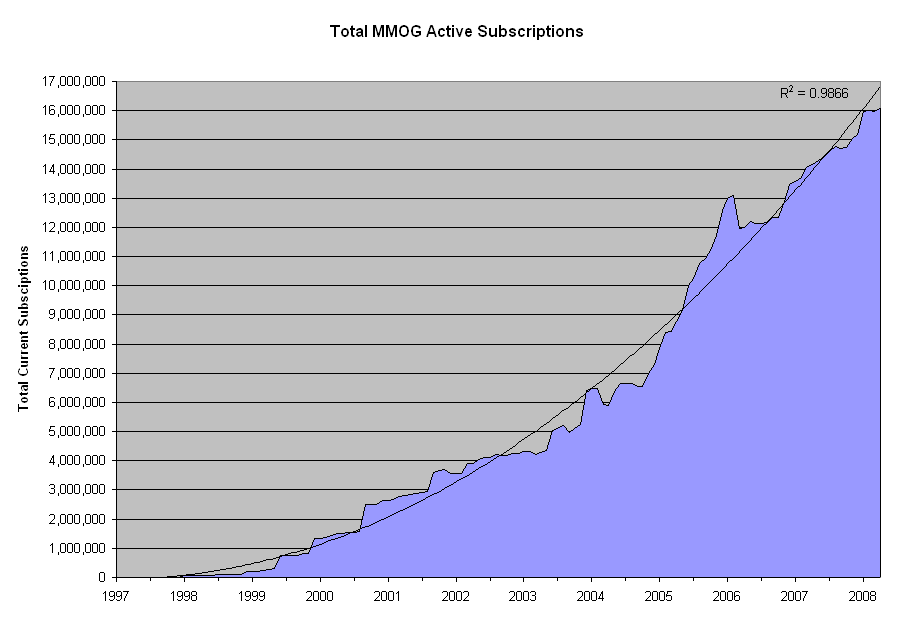
\includegraphics[width=0.7\columnwidth]{MMOG_subscriptions}
 \caption{Total number of active MMOG player subscriptions over time \cite{mmo_growth_chart}.}
 \label{fig_mmog_subscriptions}
\end{figure}

\acp{MMOG} are characterised by expansive worlds, where a large number of players interact online with each other and the virtual environment to achieve certain goals through collaboration and teamwork. Throughout the development of \acp{MMOG}, role play has been tightly coupled to this type of game. This is perhaps due to the exploration and player interaction aspects. Role play allows players to fully immerse themselves in the game world and might, therefore, provide for a more compelling experience. Because of this tight coupling, the terms \ac{MMORPG} and \ac{MMOG} have almost become synonymous. Throughout this work, a distinction will, however, be made between the two.

\acp{MMOG} hold great commercial as well as academic value. From a commercial perspective, the growing number of active subscriptions shown in Figure \ref{fig_mmog_subscriptions} translates to a growing \ac{MMOG} market. Figure \ref{fig_mmog_market} shows the online games market forecast by DFC Intelligence, a company specialising in game market forecasts for various sectors.
%
\begin{figure}[htbp]
 \centering
 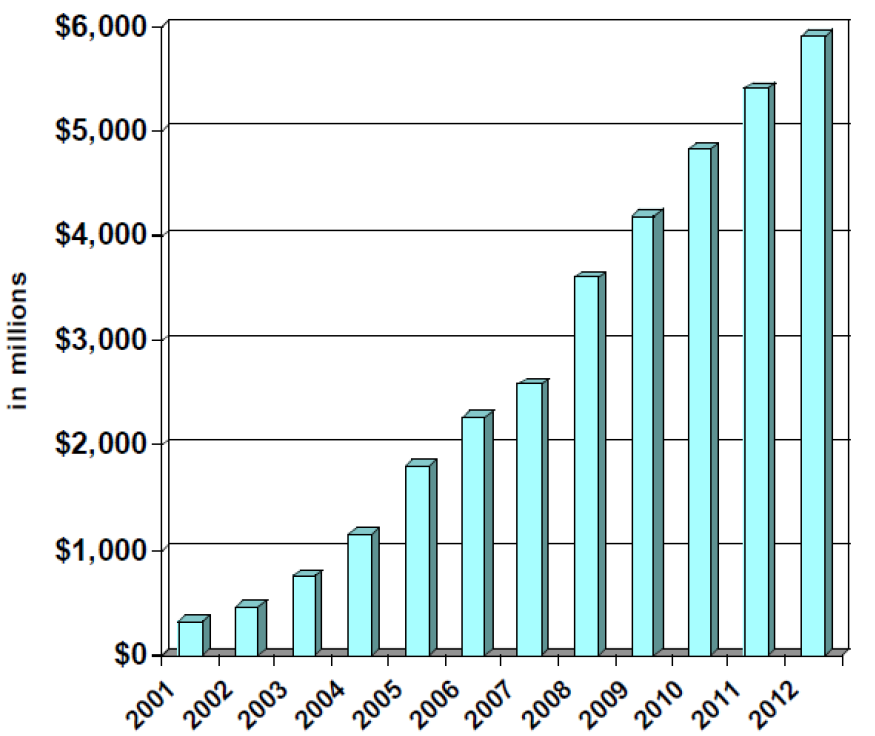
\includegraphics[width=0.4\columnwidth]{DFC_MMOG_market}
 \caption{DFC Intelligence MMOG market forecast '08 \cite{Fan_phd}.}
 \label{fig_mmog_market}
\end{figure}

From an academic perspective, \acp{MMOG} also hold great value. An MMOG is a complex networked application, with clients requiring reliable real-time feedback on actions taken. The design of an MMOG requires in-depth knowledge of server architectures and network design. The design of a server architecture determines how may players the game will be able to host and what the user experience will be in terms of quality of service. The server architecture must be able to handle thousands of requests, store large amounts of data, update the game state and send responses back to all clients in real time.

%Complete Introduction

\section{A brief history of MMORPGs}

\acp{MMOG} have a history stretching from 1978 to the present. A complete history of \acp{MMOG} and the histories of the games and boardgames that they originate from can be found in \cite{mmog_past_present_future} and Chapter 1 of \cite{designing_virtual_worlds}. The first games that could be called \acp{MMOG} were \acp{MUD} (1978) \cite{mud_intro}. \acp{MUD} are entirely text-based, with players exploring areas by receiving descriptions of what they were ``seeing'' and typing commands to move and interact with objects or players. \acp{MUD} contain many of the elements that today are still central to the \ac{MMOG} concept. These elements include exploration, large worlds, multiplayer, social interaction and progression.

After \acp{MUD}, there were many \acp{MMORPG} that acted as building blocks for what is recognised today as being an \ac{MMORPG}. The first graphical \ac{MMORPG} was Neverwinter Nights (1991) \cite{nwn_aol}. Neverwinter Nights was not an Internet based game, it was hosted on what today is the AOL network. Meridian 59 (1994) was the first \ac{MMOG} to have featured a monthly subscription fee, receive wide media coverage and most importantly, the first \ac{MMOG} to feature a 3D engine \cite{meridian59_hist}.

The first \ac{MMORPG} to be commercially successful and largely credited with popularising the genre was Ultima Online (1997). Ultima Online used existing intellectual property from the Ultima universe as well as an aggressive marketing campaign by game publisher EA, to quickly gain 100,000 subscribers. NCsoft's Lineage (1998) looked similar to Ultima Online, but was more \ac{PvP} oriented and with an added castle siege mechanism, became very popular in South Korea. Lineage had more than three million subscribers at one point, most of them from South Korea \cite{mmog_subscriptions}. Everquest (1999) is credited for bringing \acp{MMORPG} into mainstream Western Culture. It featured a large persistent 3D environment that was capable of hosting up to 15000 players per server \cite{everquest2_capacity}.

\acp{MMORPG} in the first millennium are considered to be of the first generation. These games provided blueprints for all \acp{MMORPG}
to follow in the second generation. While there are many more games in the second generation, these games are characterised by little innovation
in the genre and focus more on improving graphics and ease-of-use \cite{mmog_past_present_future}. Notable games in this generation are: Final Fantasy XI (2000) (console based), Dark Age of Camelot (2001) (realm vs. realm combat) and Anarchy Online (2001) (instancing).

Eve Online (2003), developed by CCP Games in Iceland, brought many new innovations to the \ac{MMORPG}. It was the first successful MMORPG to feature a science fiction theme. It was the first MMOG to have a single distributed server architecture. This meant that no sharding was required. Sharding is a method by which the game world is duplicated onto multiple servers to distribute load. Players cannot communicate between shards as these worlds are complectly isolated from each other. By employing a distributed server architecture, where different regions of the virtual world was hosted on different servers, players could have a seamless and more immersive experience. This was accomplished by hosting different star systems on different servers. Players have to use a warp gate to travel between star systems. This mechanic is used to mask the time it takes to move the player from one server to another. In 2006, CCP Games launched the largest supercomputer in the gaming industry to upgrade their existing infrastructure and enable Eve to support more than 50,000 concurrent users \cite{eve_launces_supcom}. This number that was surpassed in 2009 with 54,181 concurrent users in game \cite{eve_pcu}.

Another innovation of Eve was the in-game economy. CCP games appointed Dr. Eyj\'{o}lfur Gu\~{o}mundsson as chief economist of Eve online in 2006 \cite{eve_economist}. His duties were to monitor and predict market trends in the game world and produce detailed quarterly economic reports \cite{eve_econ_rep}.  The economy is based on a open market system ruled by supply and demand. No other game has implemented an in-game economy in such a rigourous fashion.

Blizzards's \ac{WoW} (2004) is the most successful MMORPG to date. After six years it still has by far the most subscribers of any MMOG, totaling 11,5 million, each paying \$15 per month subscription \cite{wow_subscibers}. In 2008 it was estimated that WoW holds more than 60\% of the MMORPG subscription market \cite{mmog_sub_market}. From the first generation of games, a steady growth has been seen in the MMOG space, but before the run away success of WoW, no one had estimated that the gaming market could be this large \cite{mmog_growth_analysis}. It should be noted, however, that the growth seen in the \ac{MMOG} market, is mostly due to growth in the Asian markets and that the size of these markets are much larger than the size of the Western markets.

The success of \ac{WoW} has largely been attributed to the overall quality and finish of the game \cite{wow_gameplay}. It is interesting to note that WoW is not attributed with many innovations. Most games that came before it implemented most of the features in WoW. What WoW did do, is combine all previous innovations into a package that was accessible to a large number of people.  Players also don't just play WoW to experience the game content, they also play the game to meet up with friends and socialise. Guilds are also an integral part of WoW. Guilds are collections of players that choose to play together to achieve some common goal.

\section{Overview of MMOG architectures}

\subsection{Networking models}

The previous section presented a brief history of the \ac{MMOG} and more specifically, the \ac{MMORPG} genre. This section explores the network architectures that are generally employed by this genre of games. The network architecture of a system specifies how the different entities in the network communicate, where authority lies and whether a centralised or distributed approach is followed. Currently, all MMOGs being operated run on a \ac{CS} architecture or a distributed \ac{CS} architecture, also called a \ac{CMS} architecture. The simplest form of network architectures used in MMOGs is the pure \ac{CS} model.

\begin{figure}[htbp]
\centering
 \subfloat[Client/Server]{\label{fig_cs_arch}
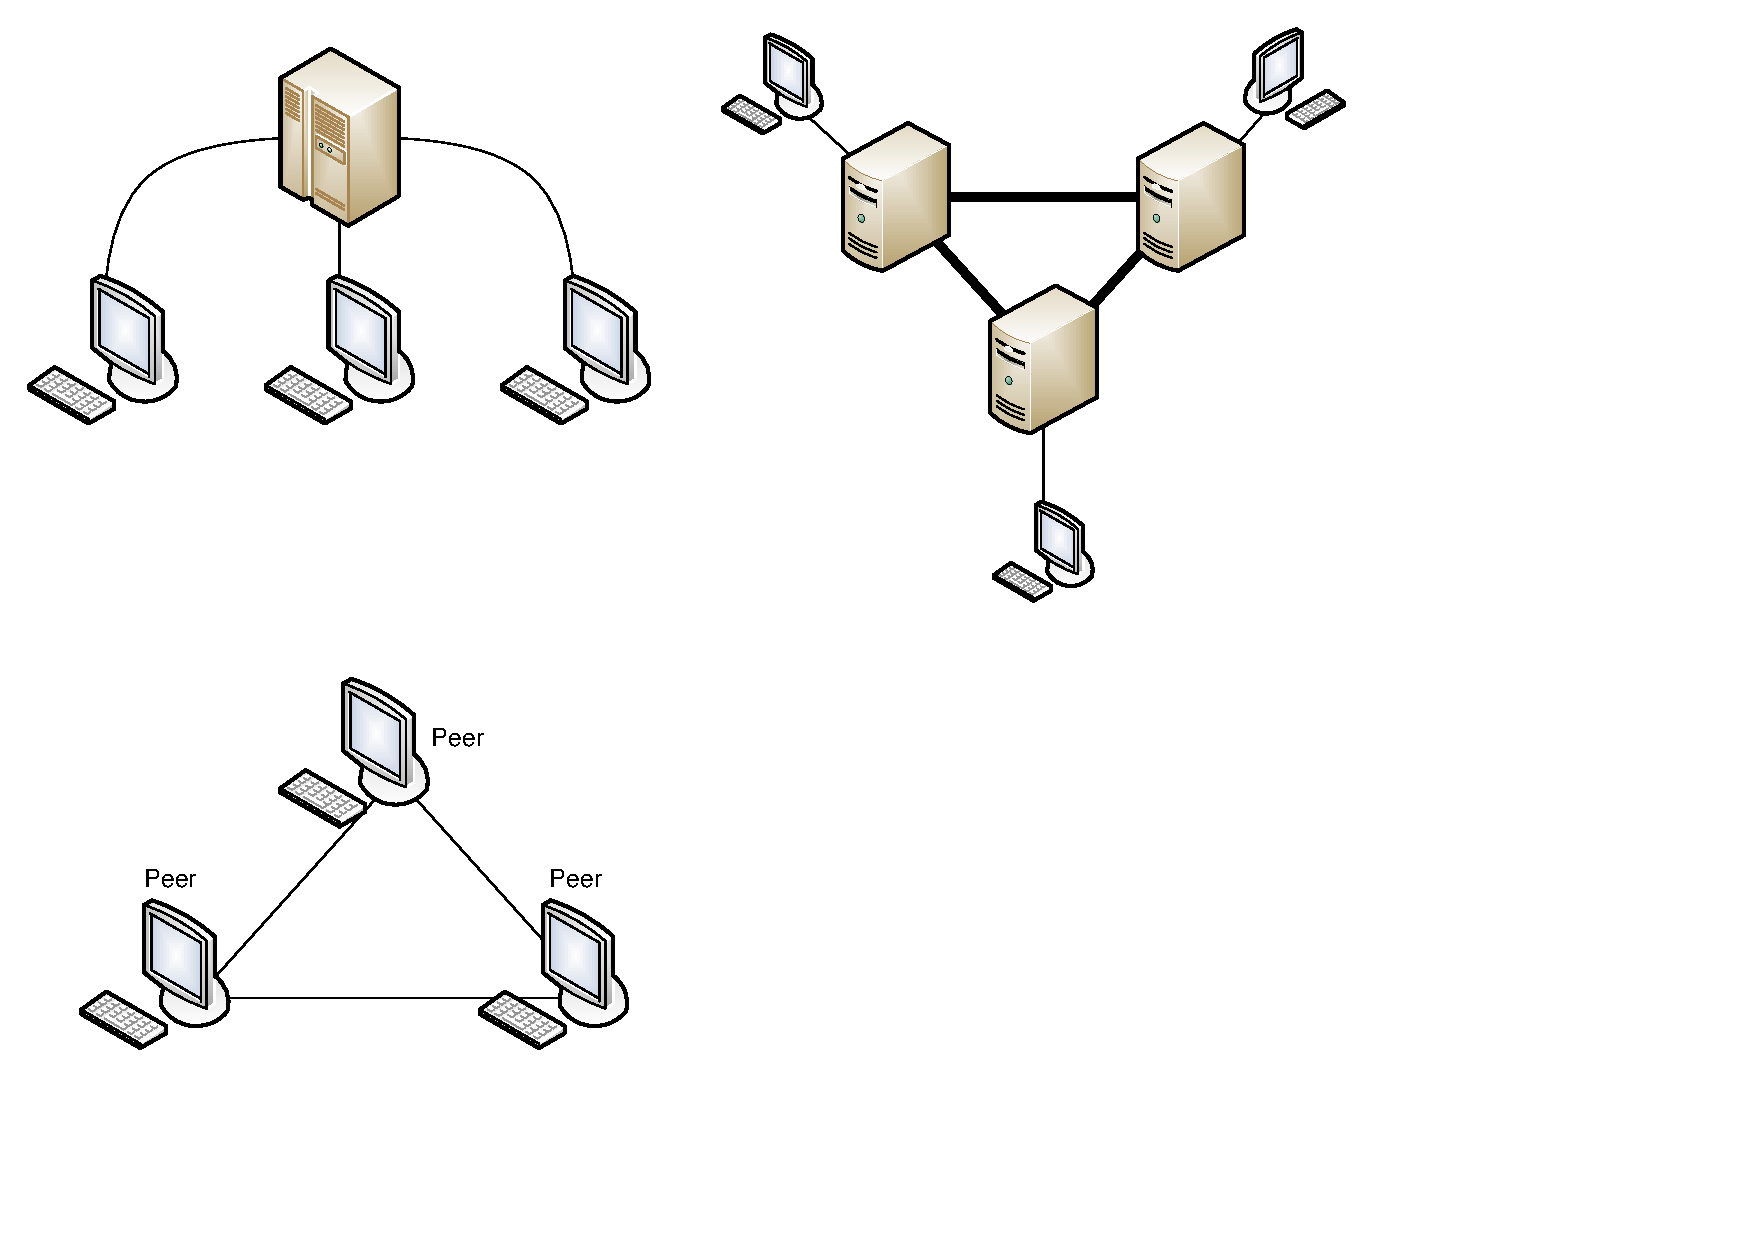
\includegraphics[clip=true, viewport= 0cm 12cm 11.5cm 21.5cm, width=0.5\columnwidth]{network_archs}}
\subfloat[Client/Multi-Server]{\label{fig_cms_arch}
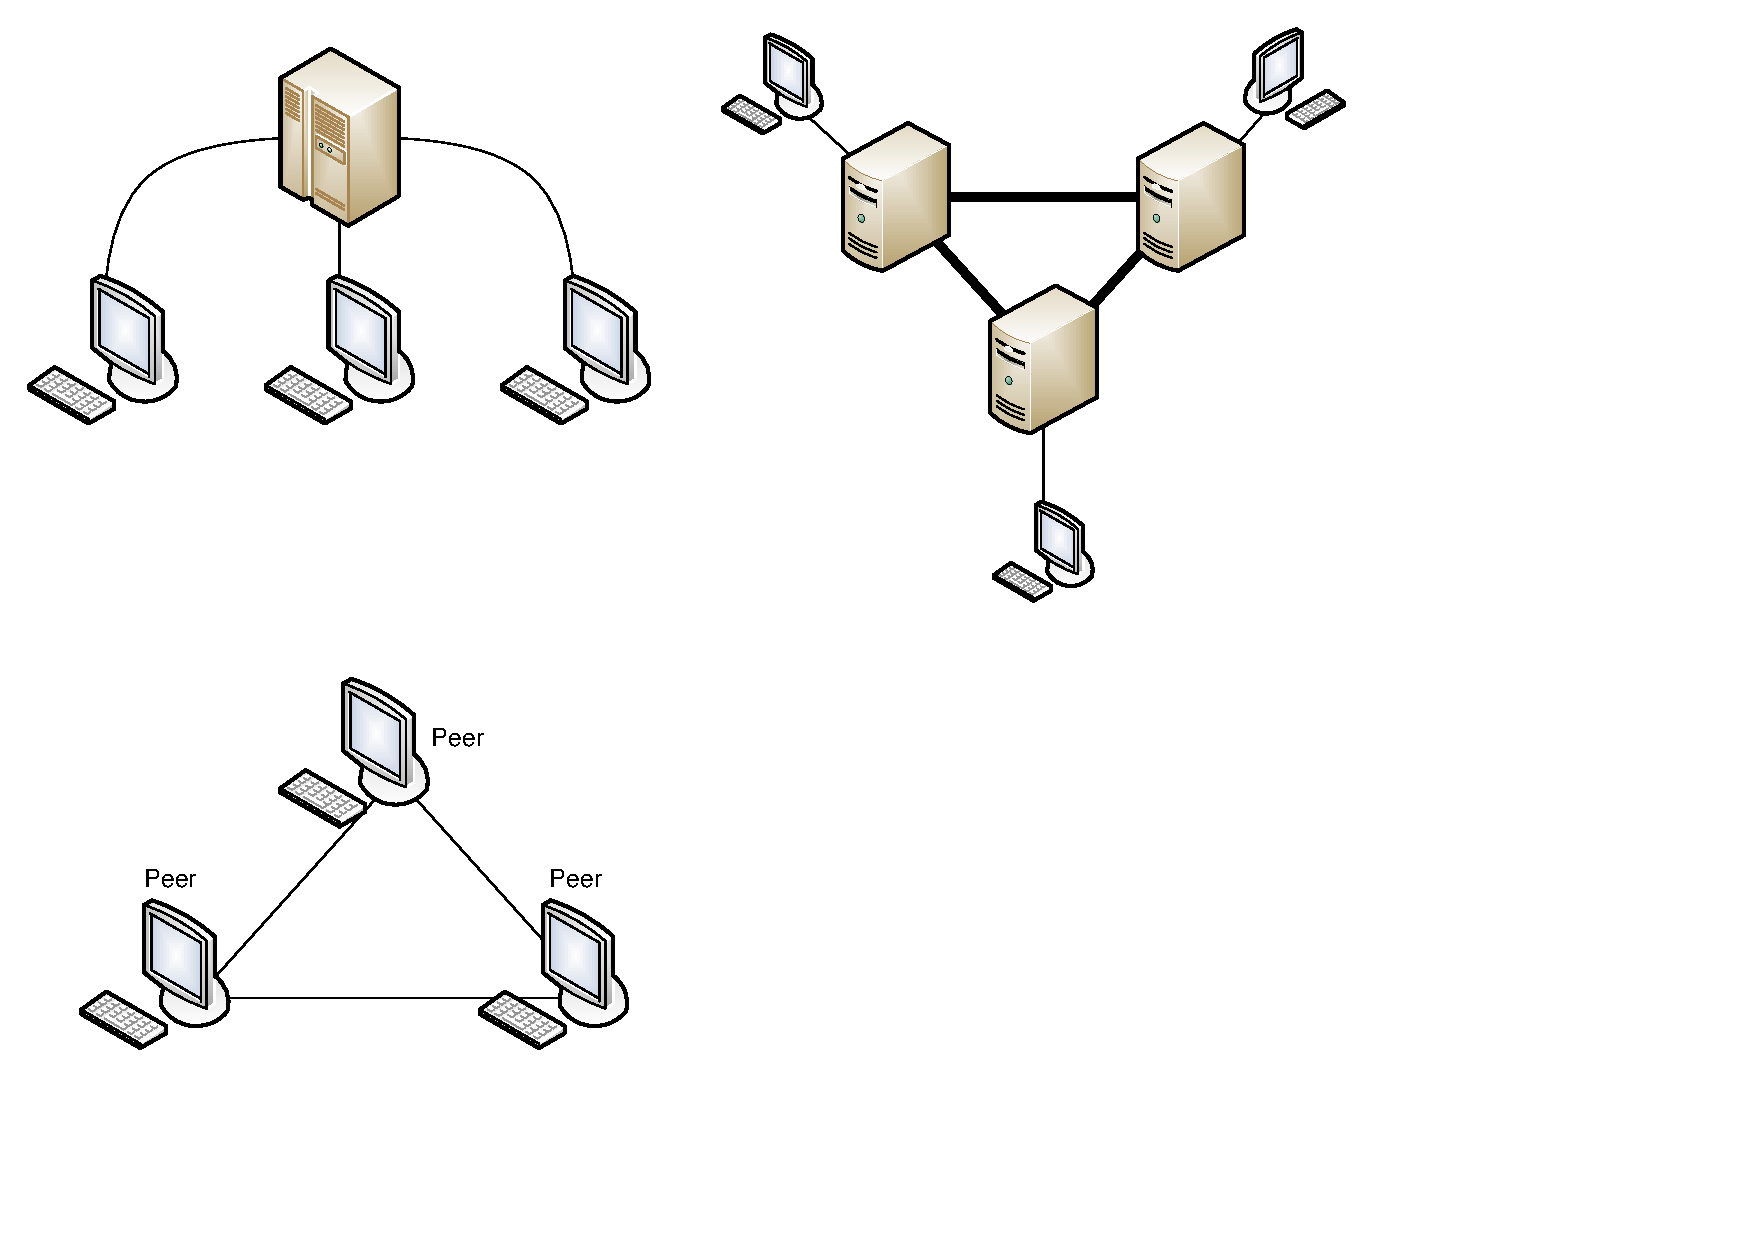
\includegraphics[clip=true, viewport= 12cm 10.5cm 23cm 21cm, width=0.5\columnwidth]{network_archs}}
\caption{Network architectures}
\end{figure}
%
Figure \ref{fig_cs_arch} shows the \ac{CS} model. The server is the entity on which the MMOG is hosted and is controlled by the game producer. Clients are computers operated by players, that connect to the server to play the game. The server is responsible for updating the game state, according to client actions, to store the new game state and to distribute game state updates to all clients. An in-depth exploration of consistency models, of which this theory forms part, will be presented in Section \ref{consistency_models}. Clients never communicate with other clients. They send their actions to the server and receive the updated states of other players from the server.

The \ac{CS} architecture has two main advantages that made it the architecture of choice for all MMOG developers. Because of the centralised approach of the architecture, both administration and security are greatly simplified. Administration is simplified, because the game producer has full control over the server, server data and code. It controls physical access as well as which clients are allowed to connect the the system. Efficient logging is also supported, because the server is able to not only log all server actions, but also all client actions, since these also pass to the server.

Security is a significant issue in MMOGs, since some players sell in-game currency for real-world currency \cite{chinese_gold_farmer}. This makes the MMOG a platform that is capable of producing income, which increases the incentive of players to be able to gain an unfair advantage over other players. The more popular an MMOG, the greater the security threat. Because the producer has full control over the server code and is never required to furnish the client with the server code, it makes it difficult for a potential attacker to use knowledge of the server in an attack. Because clients are never allowed to communicate, all malicious users can be filtered out of the network by the server when detected and even banned from the network. Producers are able to ban players, because these games usually require a game account, which is linked to a copy of the game as well as some payment method. This introduces a large cost to players whose accounts are banned.

The \ac{CS} architecture however does have some disadvantages. These are weak robustness, weak scalability, high cost to the provider, high latency, high amount of required server bandwidth and weak handling of transient loads. The robustness of the system is weak because it is a single point of failure. If the server fails or goes down for maintenance, the game is off-line and players are unable to play.

This system is also not scalable, since a single server cannot easily be extended with more resources. Even if an off-line approach is used, where hardware is upgraded after the system is taken down for maintenance, the hardware required to support a game hosting more than 3000 players, become prohibitively expensive. In 2004, it was estimated that an MMOG that supports approximately 30,000 players, requires 2 to 3 years to develop and costs more than \$10 mil to develop \cite{cs_mmog_cost}, \cite{igda_online_whitepaper}. With newer games using high definition graphics and the general drive in the market to improve on previous titles, the cost of MMOG games can only be expected to increase.

The server hardware should be able to support peak system loads, which means that sufficient resources should always be provisioned to support these peak load. This is not an economically viable solution, because resources to handle peak loads are not used most of the time. This translates to producers paying for the provisioning of resources, without having active players that pay for these resources.

This disadvantage also leads to a high cost for the provider, which translates to high costs for clients or reduced profit. The cost come from the hardware that is required to host the system as well as maintenance and running costs. Running costs include bandwidth provisioning and IT personnel and maintenance costs include replacement of malfunctioning or outdated hardware. It has been estimated that maintenance and running costs consume approximately 80\% of game revenue during the lifetime of the game \cite{cs_mmog_cost}.

Because no clients are allowed to communicate with other clients, every change that is made to the game world by a client, first had to be communicated to the server, which in turns relays this message to all clients after applying game logic and artificial intelligence (AI) algorithms. This two hop path, with the additional time for computation added by the server as well as possible buffering at the server when many clients communicate, significantly increases the latency of the system compared to a system where direct communication is used.

\subsection{Consistency models}

In an effort to address some of these issues, the distributed \ac{CS}, also called \ac{CMS}, was introduced. In a distributed \ac{CS} model, shown in figure \ref{fig_p2p_arch}, the server functions are distributed amongst multiple machines in an effort to distribute the server load. For MMOGs, there are various methods employed to achieve this. Sony introduced the first distribution method in Everquest, where copies of the game world ran on different servers and players then connect to one of these servers \cite{engineering_everquest}. Sony termed this method: ``Sharding''.

Clients are not able to interact or communicate with players on other shards, which reduces game immersion. This method does, however, allow for a more scalable system as maximum load is fixed. Players are not able to enter a shard if that shard has reached it capacity. This has in the past caused unhappiness amongst players, since popular shards could be difficult to log in to. Players are also reluctant to move to a new shard, because a lot of time is invested in their characters in their ``home'' shard. Sharding, however, wastes more resources, as one shard may be overpopulated while another is underpopulated. There is no way to dynamically distribute the available resources from one shard to another. For all practical purposes, this approach is still merely a \ac{CS} approach, with players forced into a specific \ac{CS} environment.

%Redundant
Presently, there are three popular distributed models used to enable MMOGs to scale. These are replication-based, object-based and zone-based \cite{Hu_voronoi_IM}. The first one is very similar to sharding, with the difference that all servers share the same duplicated game state. Each server contains the global game state and clients connect to any one of these servers (mirror-servers \cite{mirrored_server}) or through a load distribution algorithm to a server (proxy-servers \cite{proxy_server_dist}). Each server handles all actions from clients and updates its own database. The servers in turn send updates to each other over a high quality link, such as fibre, to maintain database consistency at high speeds. The problem with this system is that the world is never truly consistent and that there are no optimally chosen inconsistency obfuscation boundaries. In other words, two players standing next to each other in the virtual world, might be on different servers and, therefore, experience two different worlds. Game inconsistency is not necessarily an issue, but then it should be based on a distance based approach where the consistency degrades gracefully the greater the distance between players in the virtual world. This system is also not truly scalable because of the large hardware costs involved in the system as well as network hardware required to achieve sufficient performance for large numbers of players.

%Object based
The object-based method distributes all in-game objects amongst the servers \cite{object_based_consistency1}, \cite{object_based_consistency2}, \cite{object_based_consistency3}. For an MMOG, most of these objects are expected to be players objects. The advantage of this method is that the system load is fixed for a certain player population and that the load is equally distributed amongst all server. This allows for more accurate prediction and provisioning  of required resources, but still does not handle transient loads well. Another issue is inter-server communications for this architecture. The inter-server communications are random and also much more than the inter-server communications for a region based system. The reason for this is that the amount of player interaction increases with a decrease in the distance between the players. Players playing together move together, chat and interact with \acp{NPC} together. For a region based model, all player-neighbour interaction remain in the server.

%Zone-based
The zone-based method divides the virtual world into zones or regions, which are hosted on different servers \cite{zone_based_stat}, \cite{zone_based_dyn}. Busy regions are hosted on their own servers, while multiple quiet regions are hosted on a single server. This is termed the static region approach \cite{zone_based_stat}. The issue of this static region approach is that it does not scale well when one region is suddenly populated with players. This type of behaviour happens quite regularly and is known as flocking \cite{flocking}. When players find something of interest in a region, many players will flock to that region. In-game events and festivals are also becoming popular and these events also cause flocking to the region where the event is held. The solution to these effects have been over provisioning of resources to handle peak loads, which suffers from the disadvantages discussed above. Also, if the load changes, the server has to be brought off-line in order to balance the regions. Dynamic regions are being investigated, where regions can be dynamically shifted from one server to another, in order to balance load \cite{zone_based_dyn}. This approach adds overhead and significant complexity with regards to the migration of the data and the handling of player actions while the data are in transit.

In general, the issues addressed and improved by the \ac{CMS} architecture are robustness, scalability, and peak load handling. The system is more robust, because the failure of one server will not necessarily lead to the failure of the whole system for certain system designs. The system is more scalable, because many less powerful servers may be used, which allows for the hosting of more players than what is currently possible with single server hardware. It also handles transient loads better, because, for cases where loads can be predicted, resources can by shifter between servers to improve the user experience.

The disadvantages of this system is that the administration complexity is greatly increased. Such systems, although capable of handling many more users than a single server, is also much more expensive. These disadvantages are however not technical problems and so it is assumed for current games, that these systems are what is required if a game is to be hosted for a large number of players.

\section{Peer-to-Peer MMOG architectures}
\subsection{Overview}

Recently, an alternative architecture has gained popularity, making use of a peer-to-peer architecture to host the MMOG. This idea was first formally published in \cite{knutsson_p2p_first}. This has opened up a new research field that is attempting to make the peer-to-peer model a viable alternative to the classic \ac{CS} and \ac{CMS} architectures. This architecture does, however, still have a few major issues that need to be solved before MMOGs can be developed that use it. If these issues, which are later discussed, can be solved, a \ac{P2P} architecture holds some powerful advantages over a \ac{CS} system.

The core idea of the \ac{P2P} model is that each peer contributes enough resources to the network to be able to host itself. This also means that all functions of the server in the classic \ac{CS} model are distributed amongst all peers. There are many areas where the \ac{P2P} model can improve on the classic \ac{CS} model. These areas are robustness, scalability, provider cost, latency, server bandwidth and handling of peak transient load.

The system is very robust, because there is no server that can fail, only individual peers. Individual peers failing will not affect any other peers other than the peer that failed. This behaviour makes game down-time extremely unlikely.

Also, because every peer is expected to add sufficient resources to the system to host itself, this makes the system very scalable with no extra costs being incurred from a provider viewpoint for any peer that joins the network. This will also allow for efficient handling of transient loads. If many players suddenly enter the game, no resource provisioning issues will arise, as peer bring the resources they need with them into the system. It should also be noted that it is not at all unreasonable that a peer will have sufficient resources to host itself. Peer computers are very powerful systems these days, with multi-core CPUs, multiple gigahertz of clock speeds, multiple gigabytes of memory and secondary storage space in the terabyte range. The graphics cards in gaming machines have also become immensely powerful. With such a system in mind as the average gaming system, it is not unreasonable to assume that sufficient resources will be available.

\ac{P2P} architectures also create a lot of opportunity for independent developers, because a large initial investment is now no longer required to purchase the expensive server hardware. Not just are hardware costs greatly reduced, but running costs are also greatly reduced. The bandwidth required by the game server is now shared amongst users. Which means that no bandwidth costs will be incurred by the provider. Also, the amount of required bandwidth per user is usually not high, which means that users will not be expected to use a much greater amount of bandwidth.

Latency is also improved, because it is now possible to directly communicate between peers and not necessary to go through a server for communications. There is also no single server that has to process peer actions. Peer actions need only be processed by other peers who find the specific peer actions of interest. The distribution of the load as well as direct communication will reduce latency.

\begin{table}[htbp]
\centering
\begin{tabular}{|r|c|c|c|}
\hline
Property & Client/Server & Client/Multi-Server & Peer-to-Peer\\
\hline
Administration & Simple & Challenging & Complex\\
Security & High & High & Low\\
Robustness & Low & Medium & High\\
Scalability & Low & Medium & High\\
Provider cost & High & Very high & Low\\
Latency & High & High & Low\\
Server bandwidth & High & High & None\\
Peer bandwidth & Low & Low & Medium\\
Peak transient load handling & Bad & Medium & Good\\
\hline
\end{tabular}
\caption{Differences between Client/Server, Client/Multi-Server and Peer-to-Peer architectures}
\label{tab_archs}
\end{table}

Table \ref{tab_archs} summarises the differences between the three architectures as discussed thus far. What remains to be said is why administration and security were marked as complex and low respectively. From an administrative perspective, it is more complex to administer a decentralised system than a centralised one. The reason is that the game producer has full control over the server in the \ac{CS} architecture. The administration tools only have to control the centralised server or server cluster. For a peer-to-peer system, the server is the collection of all peers. The game producer does not have direct access to peers and so controlling these nodes become significantly more complex.

The server or cluster is housed in a secured location, where access can be controlled. As stated earlier, the server code is also protected and not accessible to potentially malicious players. These factors simplify the security of the \ac{CS} model by allowing the developers to place all intelligence in the server and move all sensitive computations to the server. Clients do not house game logic and the client state is also not authoritative. This provides the C/S model with a high level of security. P2P security issues are discussed in Section \ref{key_challenges}.

\subsection{P2P Overlays}

\subsection{Key challenges}
\label{key_challenges}

A recent article has identified six key challenges of P2P systems: Interest Management, Game Event Dissemination, NPC Host Allocation, Game State Persistency, Cheating Mitigation and Incentive Mechanisms \cite{Fan_deisgn_issues_p2p}. Currently, these are the most pressing issues to be addressed in the design of a P2P game. Each of these challenges will be described below.

%Some key requirements have also been identified. These requirements stipulate what characteristics an MMOG should poses, to be classified as such. %These are: Distribution, Consistency, Self-Organisation, Persistency, Availability, Interactivity, Scalability, Security, Efficiency, %Maintainability \cite{Schiele_p2p_requirements}.

%Describe key requirements
%Explain P2P overlays

%Describe key challenges
\subsubsection{Interest Management}
Interest management is used to determine the smallest amount of information that a peer requires, in order to present an accurate representation of the world to each player. The idea is not specific to P2P MMOGs and was already formally put forward in \cite{First_IM} and later with greater focus on a distributed environment in \cite{Whang_agent_based_IM}. The main idea is that a player has a limited visual range and a limited area around the player in which it can interact with objects. The player requires update information of all objects in this area, called the player's \ac{aoi}. AoI calculations also rely on the fact the a player's direction and velocity of movement also cannot change instantaneously and are bounded. Extensive research has been done into solving AoI problems and a comparison of techniques can be found in \cite{Boulanger_IM_compare}. The solutions range from aura/nimbus \cite{Benford_spatial_IM} to publish/subscribe \cite{zoned_federation} to Voronoi based models \cite{Hu_voronoi_IM}, \cite{Buyukkaya_voronoi_state_management} to hybrid models \cite{hybrid_IM}, \cite{MOPAR}. Generally, interest management solutions can be divided into coarsely or finely grained solutions.

Coarsely grained solutions usually divide the game world into multiple regions and when a player enters a region, it subscribes to that region's events. This is called the region-based publish subscribe model \cite{Fan_deisgn_issues_p2p}. All players in the region then receive the region's events, even for players not in their AoI. Finely grained techniques create groups of players from their \acp{aoi}. Groups of interacting players directly exchange information, so all players only receive information that is relevant to them. This has been termed the spatial model \cite{Fan_deisgn_issues_p2p}. The grain of the solution in turn determines the type of event dissemination that should be used, as described later in this section.

%Event Dissemination
\subsubsection{Event Dissemination}
Event dissemination deals with how information should be sent to peers after interest management has determined which information should be sent. The first application of event dissemination for online games can be found in \cite{first_GED}. Recently, \ac{alm} and unicast techniques of event dissemination have become popular, depending on the grain of the event dissemination. \ac{alm} is used, instead of router level multicast, because of a lack of general support for this technology at the router level \cite{ip_multicast_deployment_issues}.

ALM is used for coarsely grained interest management techniques, while unicast is used for finely grained techniques. Unicast is not used for coarsely grained techniques, because it is not scalable. For a network with $N$ nodes, $N^2$ messages are exchanges for every player action. but ALM significantly increases the message latency in the system, because messages first have to be routed over a P2P overlay network \cite{}. ALM is however preferred over unicast for large numbers of messages, because of the weak scalability.
%Check Badumna

%Cheating Mitigation
\subsubsection{Cheating Mitigation}


For an in-depth review of the security issues facing peer-to-peer system in general, refer to \cite{p2p_security_issues}. These issues are the same issues facing P2P MMOGs, with the exception of the game and application layer issues. %Check this?

Cheating mitigation has been identified as a major issue for P2P systems \cite{knutsson_p2p_first}, \cite{challenges_p2p_gaming}, \cite{lock_step_NEO}. The challenges reside in the fact that peers are not under the control of the game producer. Since all server data are distributed amongst peers, all peers have access to sections of the server data. Peers also have access to the distributed server code. One advantage that can be exploited is that no peer contains all server data and no one peer has more authority than another.

There are various security issues and these are usually divided according to the level of the protocol stack where they occur. The areas that have been identified by \cite{cheat_proof_event_ordering} and expanded upon by \cite{cheating_taxonomy} are: game level, application level, protocol level and infrastructure level. This is consistent with the generally used layered security model \cite{distributed_systems_security}. Game level cheats are ways in which a malicious player may gain an unfair advantage over other players, within the confines of the game. These cheats are usually because of software bugs and some examples are duplication and teleport cheats.

Application level cheats are where malicious players alter the game software to gain an unfair advantage. This is usually done by gaining access to the game state to which they should not have access at the current time. An example of this is map reveal cheats in strategy games. Where the fog of war is removed and the player can observe all the opponent's movements. Other cheats are sometimes used that augment the player's \ac{ui} with extra information that allows the player to make more informed decisions. It is debatable whether these additions are cheats, they are, however, considered almost essential for competitive \ac{WoW} play.

Protocol level cheats are cheats based on the different methods of communicating data across the system. These usually concern dropping, delaying of modifying IP packets to achieve certain outcomes in the game. Infrastructure level cheats concern exploiting the underlying infrastructure on which the games are built. These include hacking the hardware or P2P overlay.

As with all taxonomies, all cheats may not cleanly fit into one if these boxes, some cheats may occur over multiple levels or a cheat with a specific outcome can be implemented differently on different levels. The field of P2P security has recently received more attention than in the past and has started to bear fruit \cite{survey_p2p_game_cheats}. This is, however, an ongoing research field with many issues still open.

\subsubsection{NPC Host Allocation}
\subsubsection{Game State Persistency}
\subsubsection{Incentive Mechanisms}


\section{Proposed architecture}

We propose to develop a truly distributed P2P MMOG architecture, using hybrid techniques to improve upon current performance. The architecture will be developed to solve the six issues of P2P systems discussed in Section \ref{key_challenges}. Existing solutions to each of the six issues will be combined into a novel architecture, with the exception of state persistency. For state persistency, a completely novel approach will be followed in line with the design of the overall architecture.

At the core of the architecture will be how peers are grouped. The architecture will not use regions to group peers, but rather, make use of the flocking behaviour of players to dynamically group players into flocks or clusters. These clusters can then be used as the nodes in a clustered \ac{DHT}. Hybrid mechanisms can then be used to either interact with players at the individual level or the cluster level. Because of the flocking behaviour of players discussed in Section \ref{}, dynamic groups or regions that move with groups of players may be a better fit than static or even dynamic regions that operate on areas of the virtual world and not on how groups of players actually cluster.

For Interest Management, a hybrid approach will be followed such as MOPAR. This approach has been shown to perform better than either a finely grained technique or a coarsely grained technique. MOPAR partitions the game world into hexagonal regions and appoints ``home'' nodes to act as bootstrap nodes for each region. A home node of a region is that node whose ID is the closest match the the region ID. This allows any node to find the home node for a region. A master node is then selected for every region, whose function it is to inform slave nodes of new neighbours. All slaves nodes in a region register at their region's master node. Slave nodes send direction and velocity updates to their masters. Masters communicate directly with other masters if a node is about to enter their region. Masters inform their slaves of a new neighbour. Slaves communicate directly with each other, once identified by a master.

This direct communication reduces bandwidth usage in the network, because at this level, a finely grained interest management technique is used. The structured overlay does however assist in ensuring that all peers remain connected or able to reconnect if they have become disconnected by use of the home node.

We believe that a scheme where the regions or groups move with the groups of players will enhance the functionality of this scheme. If players are grouped more intelligently, less traffic will have to flow between groups, which will reduce the number of queries to the DHT, which in turn will improve the latency of the overall system. Using groups or flocks would, therefore, compliment this technique. The issue with such a system would be how to uniquely identify a group and how the identification would be applied when groups merge or split. The identification is required in order to ensure that disconnected nodes are able to reconnect, once they have joined a group.

As Game Event Dissemination is closely coupled to the Interest Management technique, unicast will be employed. Unicast is used between all master nodes as well as between all slave nodes in MOPAR. Unicast holds many advantages over ALM, if the number of neighbouring nodes are bound. ALM introduces significant delays into the communications system, by the use of an overlay that requires $O(\log(n))$ hops on average to route a message to a target. While $O(\log(n))$ is sufficient and indeed a good order complexity for routing, in a latency critical application such as an MMOG, this is not sufficient. Unicast, in contrast, provides an $O(1)$ routing complexity. And the fact that groups are used, allows for the unicast group size to be bound.

Security is also of great importance to the design of an MMOG architecture and so security issues will be kept in mind when designing the MMOG architecture. Recent advances and surveys can be used to improve game security, by improving the security of currently used peer-to-peer overlays. Examples include using secure node ID assignments, by making use of a Certification Authority, or designing the system in such a way that a peer cannot select or report it's own node ID. All aspects of security will be investigated, this includes Authentication, Authorisation, Data Integrity, Confidentiality, Availability, Trust, Privacy and Identity Management \cite{distributed_systems_security}. Current schemes usually only handle one or two of these requirements as will be discussed in Section \ref{current_architectures}.

%Current incentive mechanisms
Incentive Mechanisms are also of key importance in a P2P system. If peers are not required to share resources, this will lead to system degradation. Two factors should however be addressed: How will resource provisioning be incentivised and more importantly, how will this scheme be made secure. In other words, the scheme should not only ensure that resource provisioning is incentivised, it should also ensure that peers are not able to cheat the incentive mechanism, by providing false information to other peers.

The focus of this work will, however, be on game state persistency. This is an area that has not received much attention in the P2P gaming field. Significant focus has been placed on Interest Management, Event Dissemination and, to a lesser degree, on Cheating Mitigation. The proposed state persistency mechanism is discussed in detail in Section \ref{proposed_persistency}. As an overview, a distinction will be made between ephemeral data and persistent data. A peer-to-peer overlay will be used to securely store persistent data, while a distance based approach will be used to store ephemeral data in a group or flock of peers. This will allow for high speed game state updates for peers within the same group, but the structured approach will still ensure the availability of the game state to other flocks of players, to a lesser state of consistency. It is also argued that players not near to each other, do not require a perfectly consistent view of the complete world. As different flocks near each-other, the degree of state consistency will become higher until the groups merge and the sates are consistent.

It is argued that NPC hosting is merely a specialised form of state persistency. NPCs are seen as objects with logic and state, both of which are data that has to be stored. This merely requires for the definition of game state to be expanded, as elaborated upon in Section \ref{proposed_persistency}. Object logic is both something that has to be stored as well as executed. The question of how and where object logic should be executed should also be investigated.

\section{Current architectures}
\label{current_architectures}

%Remember to talk about security in P2P overlays
%Zoned warra warra

\section{Consistency models}
\label{consistency_models}

\section{Proposed state persistency model}
\label{proposed_persistency}

Game state will be defined in this work as objects with state and logic. Objects can also produce events to be sent to other

\section{Current state persistency models}

\section{Expected Outcomes}

\section{Conclusion}
The conclusion goes here.

\bibliographystyle{IEEEtran}
\bibliography{P2P_MMOG}

% that's all folks
\end{document}


